\section{Delivery System}


\subsection{Delivery Pipeline}

\begin{figure}[h]
\centering
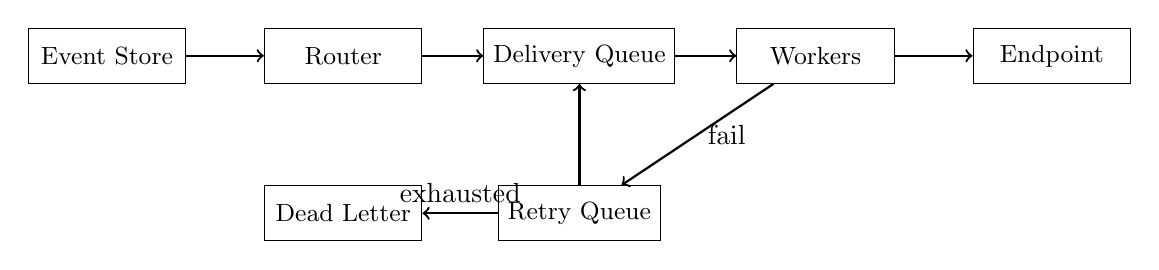
\begin{tikzpicture}[
    node distance=1.5cm,
    box/.style={rectangle, draw, minimum width=2cm, minimum height=0.7cm, font=\small},
    arrow/.style={->, thick}
]
    \node[box] (events) {Event Store};
    \node[box, right of=events, xshift=1.5cm] (router) {Router};
    \node[box, right of=router, xshift=1.5cm] (queue) {Delivery Queue};
    \node[box, right of=queue, xshift=1.5cm] (worker) {Workers};
    \node[box, right of=worker, xshift=1.5cm] (endpoint) {Endpoint};

    \node[box, below of=queue, yshift=-0.5cm] (retry) {Retry Queue};
    \node[box, below of=router, yshift=-0.5cm] (dlq) {Dead Letter};

    \draw[arrow] (events) -- (router);
    \draw[arrow] (router) -- (queue);
    \draw[arrow] (queue) -- (worker);
    \draw[arrow] (worker) -- (endpoint);
    \draw[arrow] (worker) -- node[right] {fail} (retry);
    \draw[arrow] (retry) -- (queue);
    \draw[arrow] (retry) -- node[above] {exhausted} (dlq);
\end{tikzpicture}
\caption{Webhook delivery pipeline}
\end{figure}

\subsection{Delivery Attempt}

\begin{definition}[Delivery Attempt]
A delivery attempt $d$ for event $e$ to subscription $s$ comprises:
\begin{itemize}
    \item HTTP POST to $s.url$
    \item Headers: content type, signature, event metadata
    \item Body: JSON-encoded event payload
    \item Timeout: 30 seconds
\end{itemize}
\end{definition}

\begin{lstlisting}[caption=Webhook Request Format]
POST /webhooks HTTP/1.1
Host: example.com
Content-Type: application/json
X-Webhook-Event: order.created
X-Webhook-Signature: t=1548892800,v1=abc123...
X-Webhook-Delivery: del_xyz789
X-Webhook-Attempt: 1

{
  "id": "evt_abc123",
  "type": "order.created",
  "created": 1548892800,
  "data": {
    "object": {
      "id": "ord_xyz",
      "total": 9999,
      "currency": "usd",
      ...
    }
  }
}
\end{lstlisting}

\subsection{Success Criteria}

\begin{definition}[Successful Delivery]
Delivery is successful if the endpoint returns HTTP status code in $[200, 299]$ within the timeout period.
\end{definition}

